\documentclass[oneside]{article}
\usepackage{fullpage}
\usepackage[pdftex]{graphicx}
\DeclareGraphicsExtensions{.png,.pdf}
\graphicspath{{images/}}
\usepackage{hyperref}
\usepackage{verbatim}
\usepackage[format=plain,font=small]{caption}
\usepackage[small]{titlesec}
\usepackage[round,sectionbib]{natbib}
\bibliographystyle{plainnat}
\renewcommand\rmdefault{bch}
\linespread{1.07} 

\begin{document}

\title{Glyph-maps for visualizing climate data and models}
\author{Cook, Hofmann, Wickham, Wickham}

% Drawing trend lines on map
%   - How to
%   - Comparison to coloring slope
%   - Reference to Grinstein icon plots
% Pickett RM and Grinstein GG (1988). Iconographics 
% displays for visualizing multidimensional data. 
% In Proc. IEEE Conference on Systems, Man, and Cybernetics, pages 514-19.
% Note the later work on metaphoric data display, garbage work!
%   - Alexander Gribov's work http://rosuda.org/software/Gauguin/gauguin.html

%   - Spatial star plots by Andrews http://www.udallas.edu:8080/~andrews/software/software.html
%   - Look at what Bertin does
%
% Interactive graphics
% Data processing
%
% Perhaps the GHCN data? Not gridded
% NOAA data, almost grid, but over ocean, so maps more tricky
% NARCAP from NCAR?
% Fill in with NASA data, to start, try to put new data for final version
\maketitle

\section{Introduction}

Climate data is composed of measurements on variables such as temperature, precipitation, and winds that have been collected from a spatial and temporal context. The classic display for spatial data is to use color or grey scale overlaid on geographic location, typically including a map. When measurements are made a different time periods also a common way to display the data is in small multiples, such as in Figure \ref{fig:facetted-map}. In this plot, a separate map is drawn for each month (columns) and year (rows), over a 6 year period of remotely sensed temperature data above Central America. Color is used to display the de-seasonalized temperature measurements, with red being high values and blue being low values. The data  comes from \cite{NASA-Data-Expo}. The most noticeable feature in this display is the strong red in the equatorial region beginning in mid-1997 and tapering out during 1998. This is the pattern of an El Ni\~no event, a major temperature anomaly. With some work other smaller more localized patterns can be perceived, for example, cooler over the land mass in the early year, but warmer in the latter years. What the reader is required to do is play the game "Spot the difference" from one small image to another. It's a very hard task for readers to do. Large structure such as the El Ni\~no event are clear but readers will not be able to effectively glue the images together sufficiently to read off the trend over the years or notice small local deviations between plots.

\begin{figure*}[htp]
\centerline{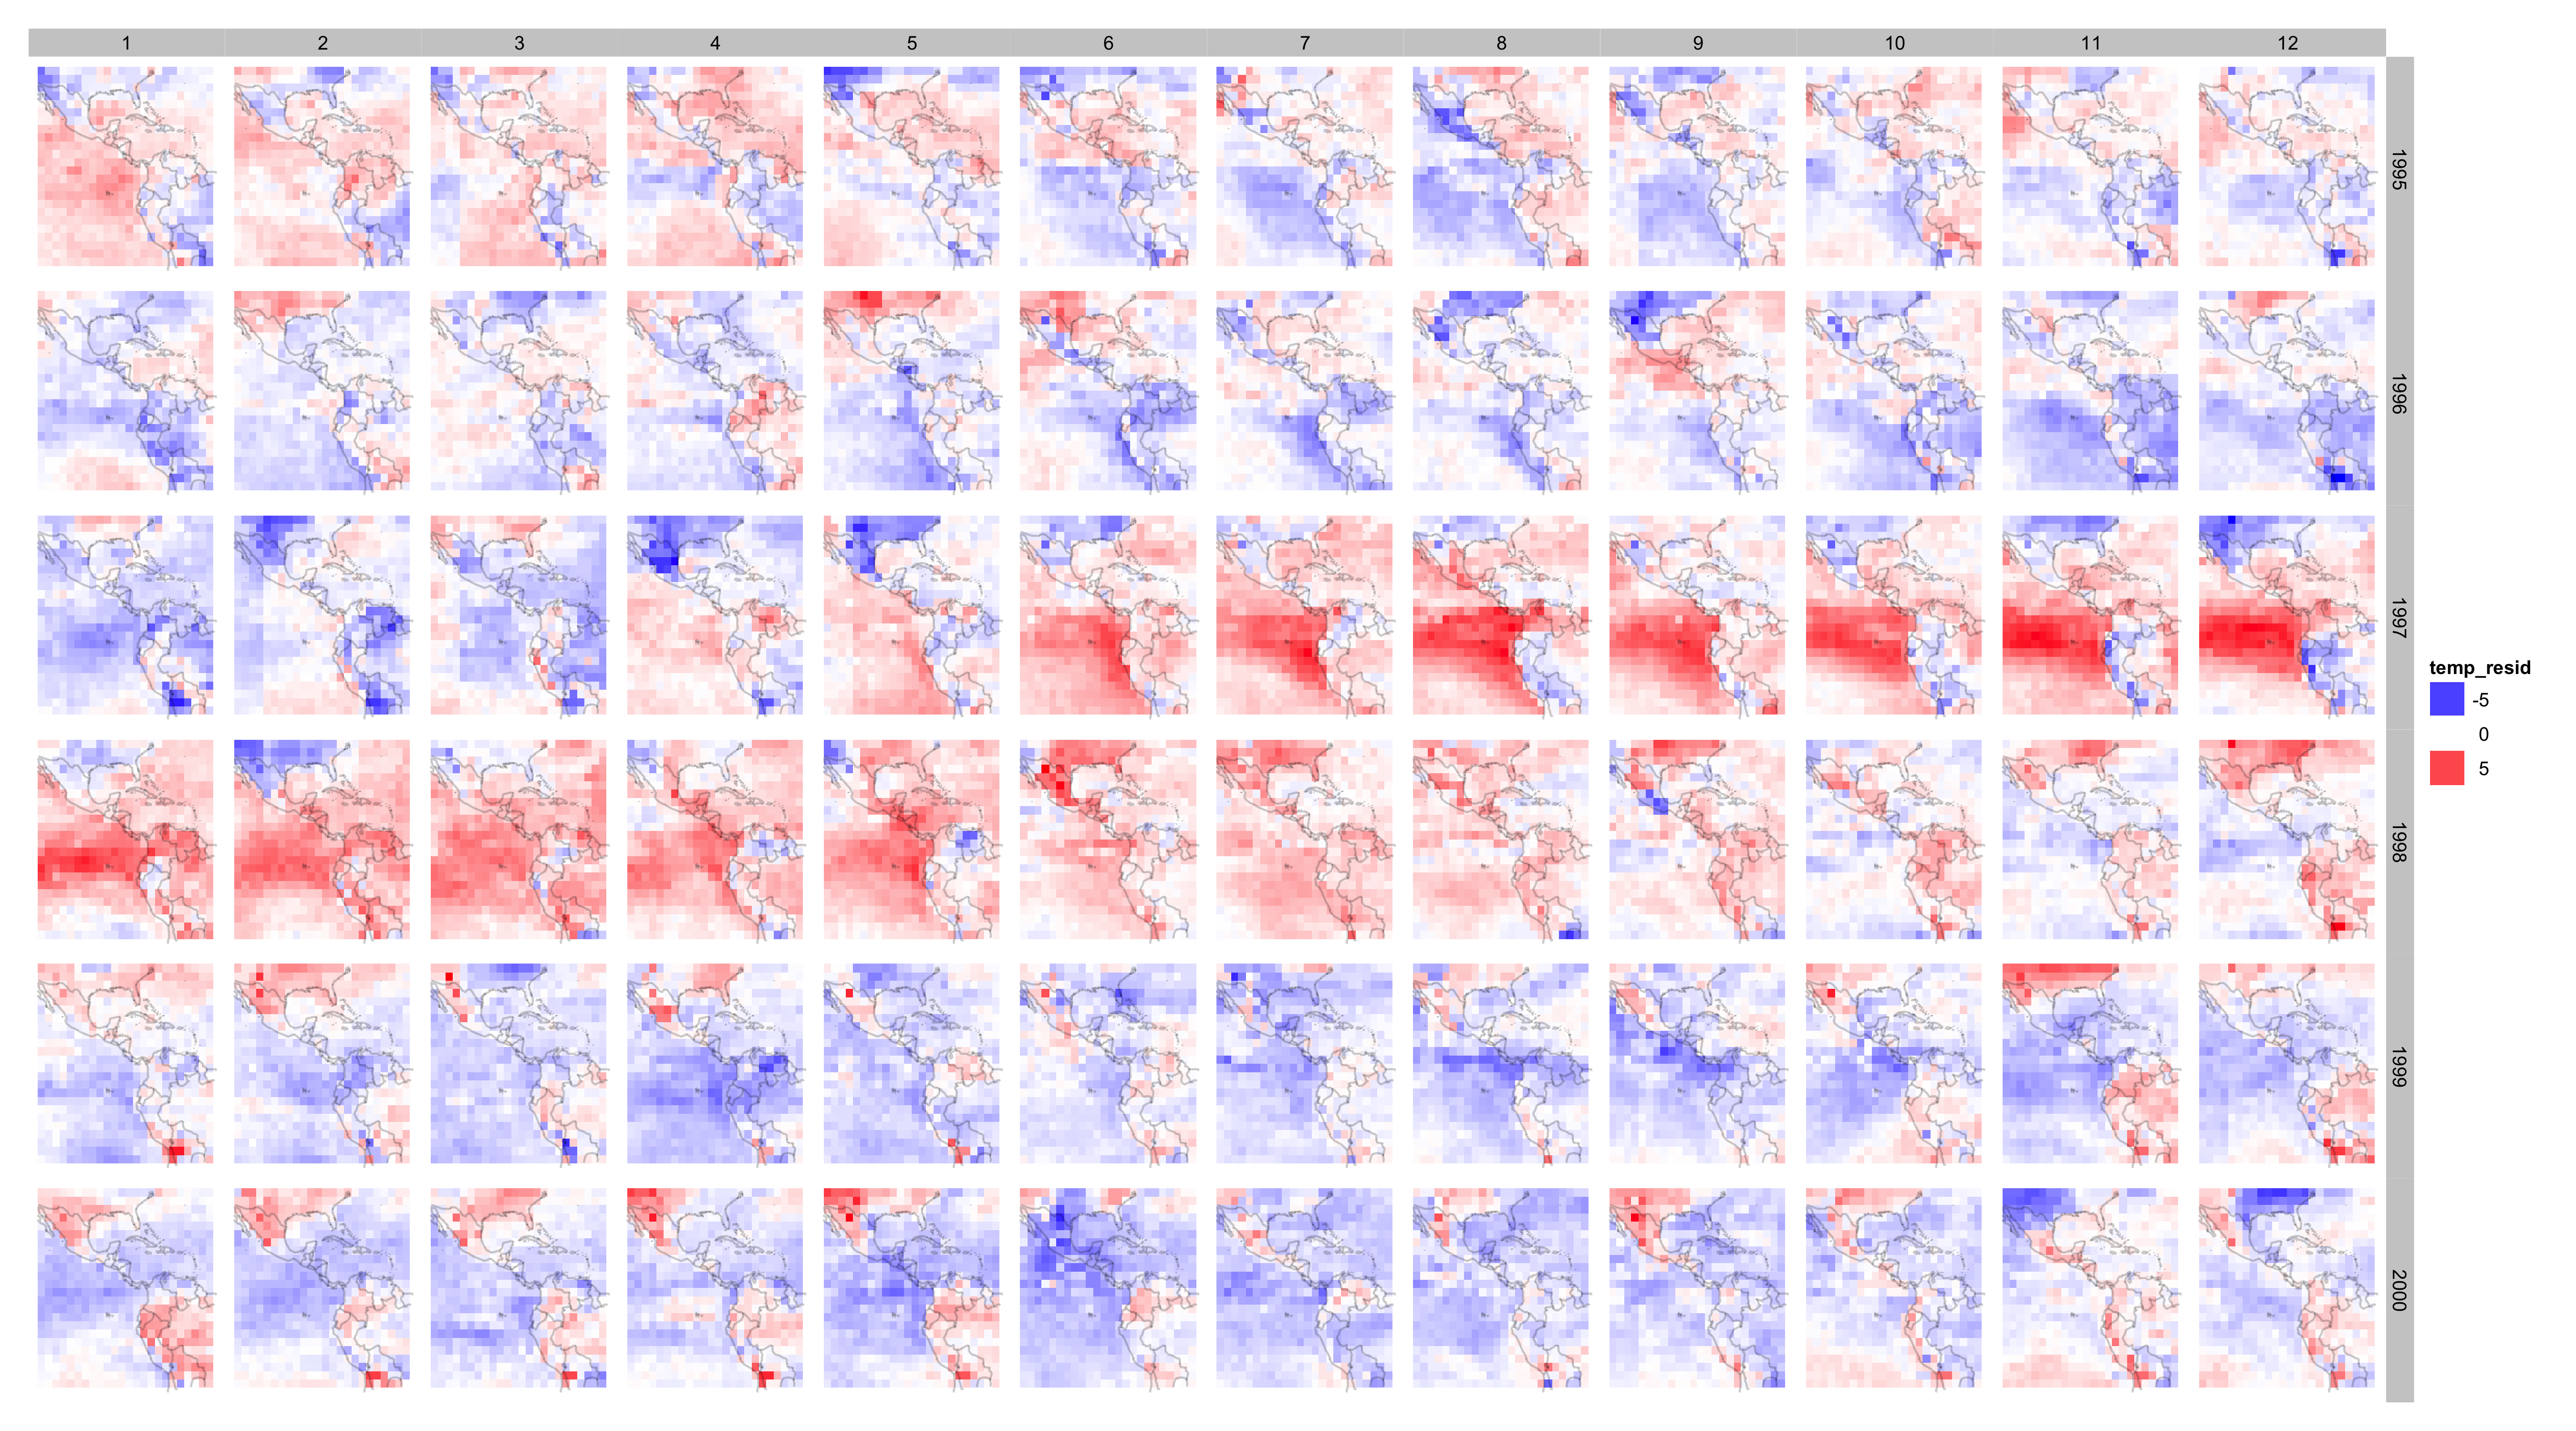
\includegraphics[width=6in]{nasa-colored-map.png}}
\caption{Facetted map of de-seasonalized temperature.}
\label{fig:facetted-map}
\end{figure*}

In this paper we explore the use of a different type of display, that uses icons on the map, for climate data. Icon plots date back to the star glyphs of  \citep{kleiner:1981}, and were made infamous by \citep{Chernoff}. An icon is produced by mapping each variable to some feature of the icon. One icon is generated for every case in the data set. Figure \ref{fig:glyphs} illustrates the idea of icon plots, with emphasis on temporal data. The time measurements are treated as variables in a multivariate data set. Here we have six years of monthly data, giving 72 time values which are considered to be 72 variables. Three different locations are selected, for demontration purposes. The top plot shows the time series of these three locations. Location ``1.1'' (red) has medium values of temperature, with strong seasonality, the six years corresponding to the six eaks. Location ``2.1'' (green) has generally high temperature values, with weaker seasonality in most years and a lack of low temperatures in the middle of the time period when lows would be expected. Location ``3.1'' (blue) has strong seasonality but generally low temperatures. The bottom plot shows these same cases as star glyphs. A separate glyph is created for each location. The 72 time variables form axes organized radially. Each temperature value is plotted relative to the overall range of temperature values. The seasonal patterns are clearly visible in this type of display, forming six ``petals'' in the icon. Location ``2.1'' has a different pattern than the other two, with only four petals, and location ``3.1'' is a much smaller ico indicating overall lower values. 

\begin{figure*}[htp]
\centerline{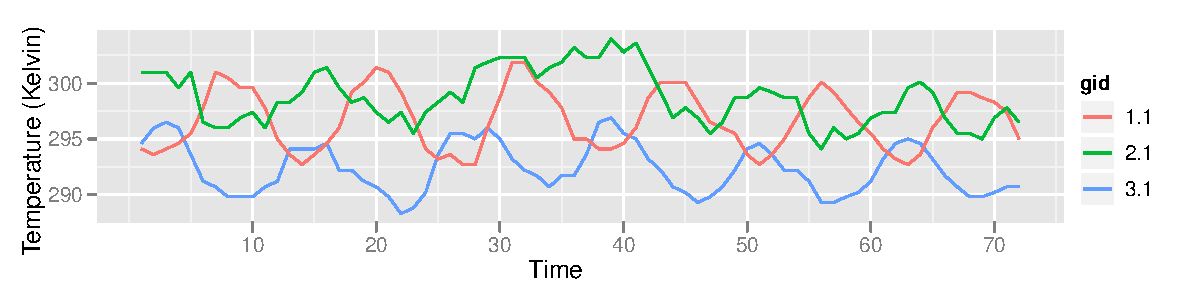
\includegraphics[width=6in]{nasa-glyph-ts.pdf}}
\centerline{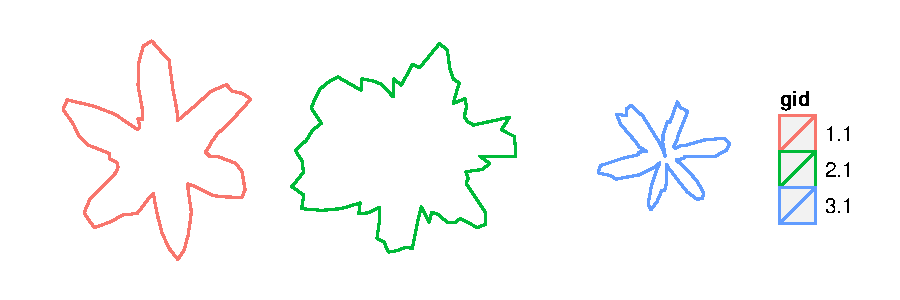
\includegraphics[width=6in]{nasa-glyph.pdf}}
\caption{Glyphs of temperature for three different locations.}
\label{fig:glyphs}
\end{figure*}

Icon plots are used, infrequently, to examine multivariate data. For large data sets it is infeasible to digest the quantity of icons, and for multivariate data there is no natural order so it can be like having a mountain of little stamps to rearrange and organize, in order to understand the structures present in the data. The initial paper on star glyphs \citep{kleiner:1981} and a recent paper \citep{hurley:2010} propose some approaches for organizing the icons. With spatiotemporal data ordering of icons is naturally done by spatial location. There is also usually some spatial trend, or continuity, which will make digesting patterns among the icons simpler.

Figure \ref{fig:glyph-map} shows the glyphs drawn for each spatial location of the raw temperature data.

\begin{figure*}[htp]
\centerline{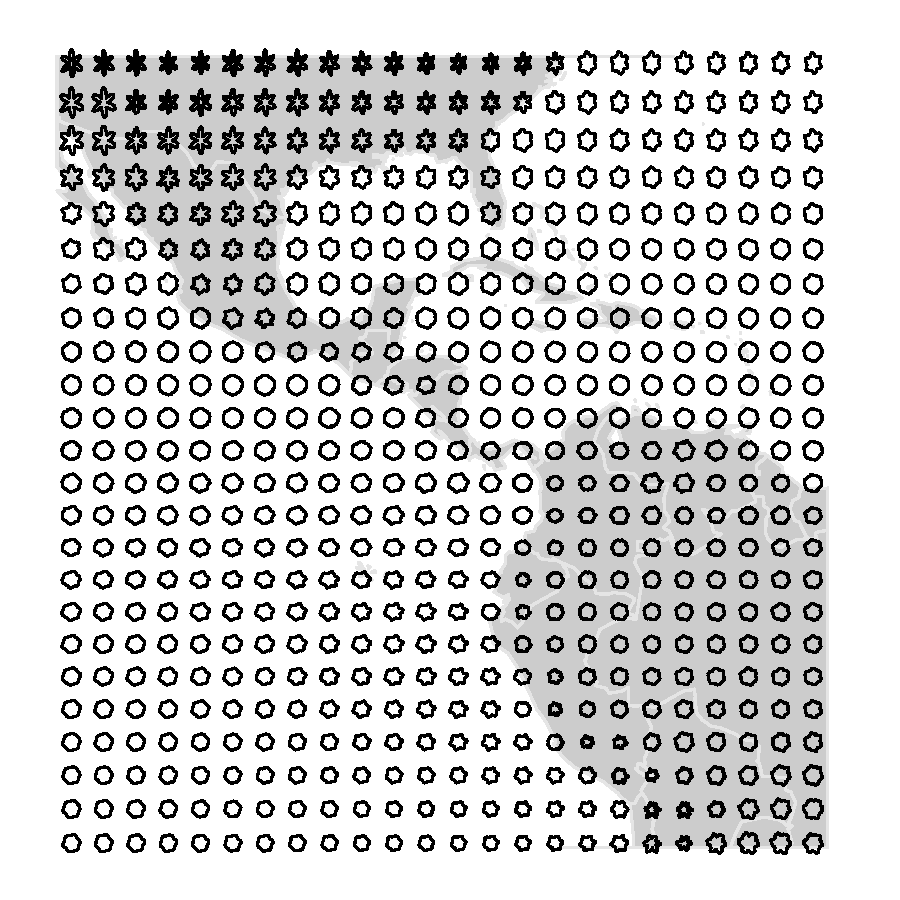
\includegraphics[width=5in]{nasa-glyph-all.pdf}}
\caption{Glyph-map of raw data.}
\label{fig:glyph-map}
\end{figure*}

%\subsection{Glyph plots}

%Simple, but effective, technique that combines aspects of glyphs, facetted plots and map-charts. Particularly well suited for the type of temporal-spatial data, commonly seen in climate.

%Glyph-maps have attributes of both glyphs (stars, faces, profiles, ...), inviting exploration at the global level, and small-multiple time series, allowing local exploration of individual series. Allow to see both geographic context and individual locations simultaneously.

%An interesting attribute of these glyph plots is that the position of graphical elements is determined by major and minor axes. For maps, the major axes are latitude and longitude, and the minor axes are typically time on the x-axis and some measurement or model prediction on the y-axis.

%Avoids one problem that plagues glyph displays: the ordering of the variables. Although some techniques exist to ameliorate this problem \citep{kleiner:1981,hurley:2010}, they are not necessary with time data because it is intrinsically ordered.

%These displays tend to be particularly effective when printed in large format, as the much higher resolution of print (600 dpi) compared to computer  screen (72-120 dpi) allows for much finer reading. These are high-density data displays in the best tradition of Tufte. Wall size maps are not usually practical during analysis, but are very engaging.

%Will first explore for regularly gridded data, a simple starting point and a common output of climate models, and then show a few simple extensions to deal with non-rectangular grids and irregular locations, as exemplified by raw climate data which is typically collect at irregular locations.
\section{Generating a time series at each location}

\begin{figure*}[htp]
\centerline{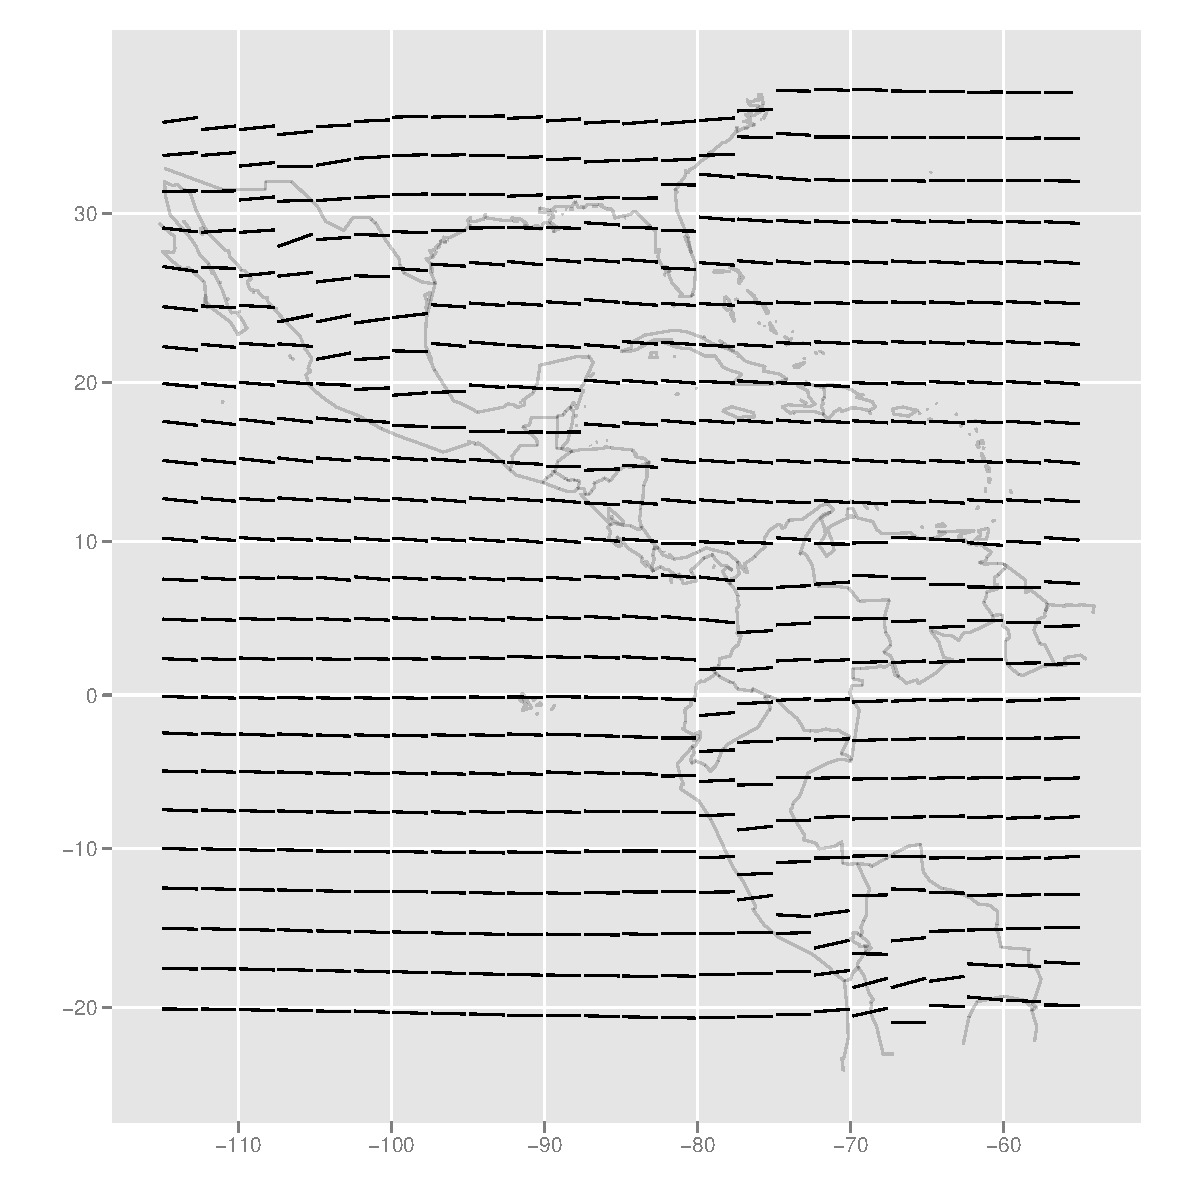
\includegraphics[width=4in]{nasa-deseas-trend.pdf}}
\caption{Time series icon at each location, showing de-seasonalized trend.}
\end{figure*}

\section{Showing seasonal effect, radially oriented icon}

A big advantage of glyph-maps is that they can be generated with existing graphics software, after a simple pre-processing step. This makes them immediately accessible to a wide audience. The graphics in this paper were created in R \citep{R} using ggplot2 \citep{me:ggplot2,wickham:2007d} and \citep{me:plyr}, but are readily implemented in any statistical programming environment.  Code and data is available in the online supplementary materials.

Because the x and y locations are linear combinations of two variables, these types of displays can also be built interactively by software that supports tours, such as DataViewer, XGobi or GGobi.  This technique is used to good effect in \citet{buja:1996a}.

\section{Reference lines}

Space-time-glyphs usually require a \emph{visual reference grid} \citet{cleveland:1993a} to make it easier to compare locations. This is important for accurate perception of important line properties like slope and minima. This need is well illustrated by Figure~\ref{}. When we add a reference to each location, as in Figure~\ref{fig:ref-basic}, we see not only a difference in shape between Northern and Southern hemispheres, but also average value. Without reference lines, it is difficult to see that average seasonal coefficients are much higher in the North than in the South.

Figure~\ref{fig:ref-basic} shows two reference grid variants: a line drawn at the overall mid-range, and a box drawn around each grid cell. We prefer using white for these references because it is minimally perceptible: you can see the grid easily when looking for it, but it does not otherwise distract from the perception of the graphic \citep{carr:1994}.

\begin{figure}[htbp]
  \centering
  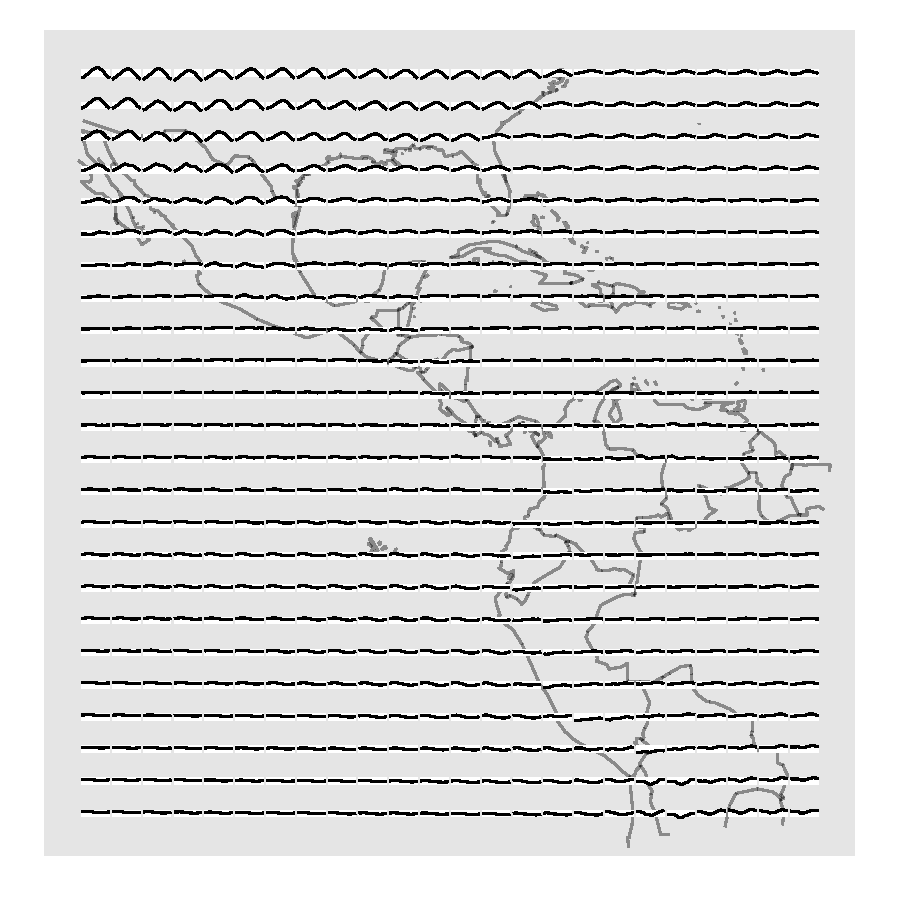
\includegraphics[width=0.5\linewidth]{ref-line}%
  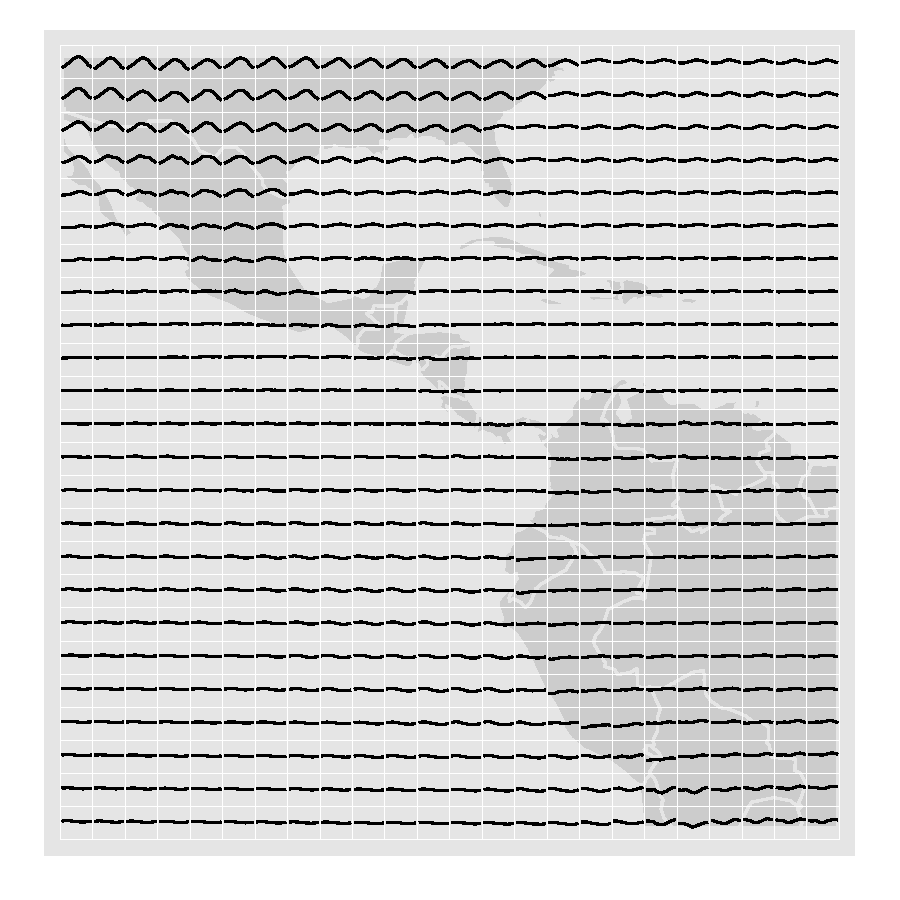
\includegraphics[width=0.5\linewidth]{ref-box}

  \caption{Glyph-maps of seasonal temperature patterns. Adding reference lines, (left) mid-range lines and (right) grid-cell boxes, makes it easier to see differences in glyph position, not just shape.}
  \label{fig:ref-basic}
\end{figure}

It's also often useful to display other types of reference information. You are only limited by your imagination (and the capabilities of your graphics software), but two simple ideas are to (1) vary the colour or transparency of glyphs or references, or (2) use an additional layer to highlight special points. Figure~\ref{fig:ref-adv} illustrates these ideas to display the month with the highest temperature at each locations. Careful colour choice is necessary so that this information is perceptible, but not distracting.

\begin{figure}[htbp]
  \centering
  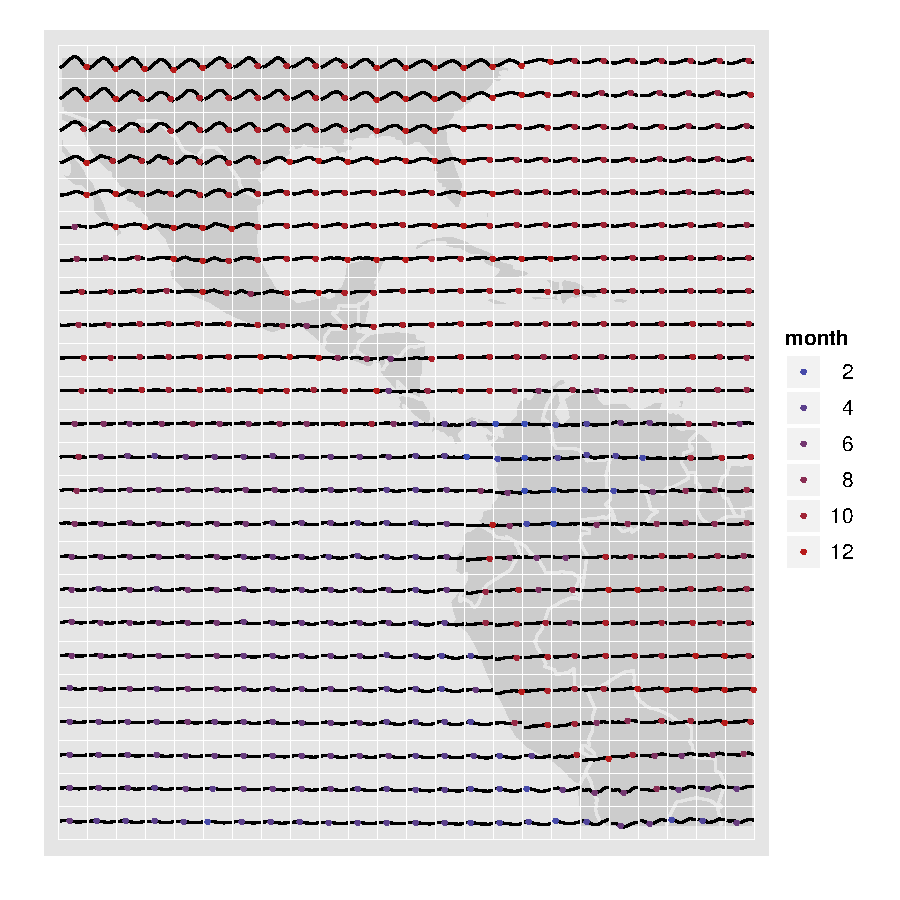
\includegraphics[width=0.5\linewidth]{ref-max-1}%
  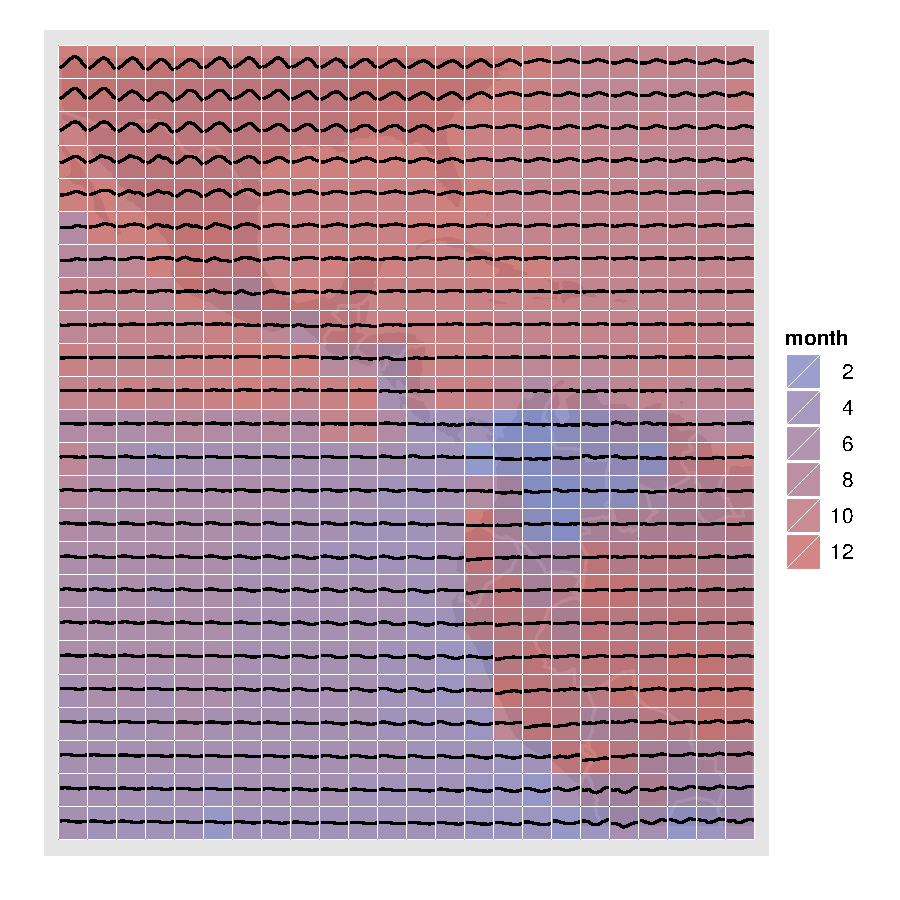
\includegraphics[width=0.5\linewidth]{ref-max-2}
  \caption{Glyph-maps of seasonal temperature patterns also showing the month with the highest temperature using (left) an additional layer of points and (right) changing the background colour of the reference grid.}
  \label{fig:ref-adv}
\end{figure}

A particularly useful summary when to add when displaying model predictions, is some measure of model fit. This makes it easier to avoid over-interpreting predictions from poorly-fitting models.

\section{Radial icons/star glyphs}

These time series glyphs can be readily altered to support circular variables, by projecting each line into polar coordinates and joining the ends. This type of display is best suited for variables that are truly circular, such as seasonal patterns or angles (such as for wind direction).

Cite star glyphs.

The alteration to the data transformation is quite simple. Without loss of generality, we assume that $y_{minor}$ becomes $r$, the radius, and $x_{minor}$ becomes $theta$ the angle, both rescaled to lie between 0 and 1. Then the glyph $x$ coordinate is given by $x_{major} + \frac{w \cdot r}{2} \cos(2 \pi \theta)$, and the $y$ coordinate by $y_{major} + \frac{h \cdot r}{2} \sin(2 \pi \theta)$.

\begin{figure}[htbp]
  \centering
  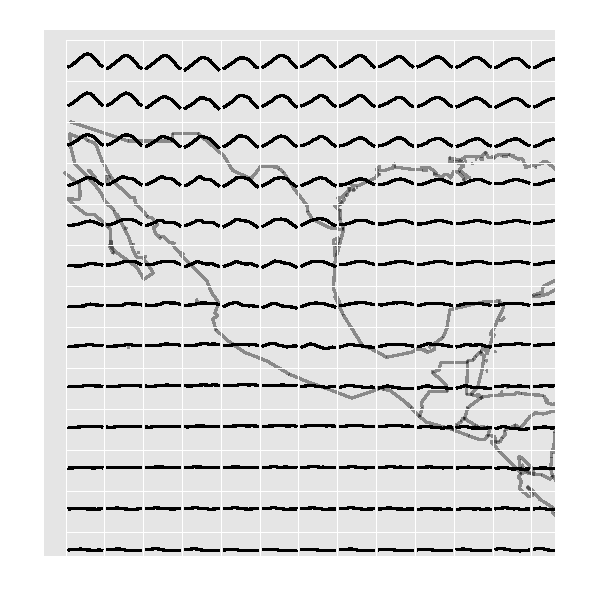
\includegraphics[width=2in]{month-cartesian}
  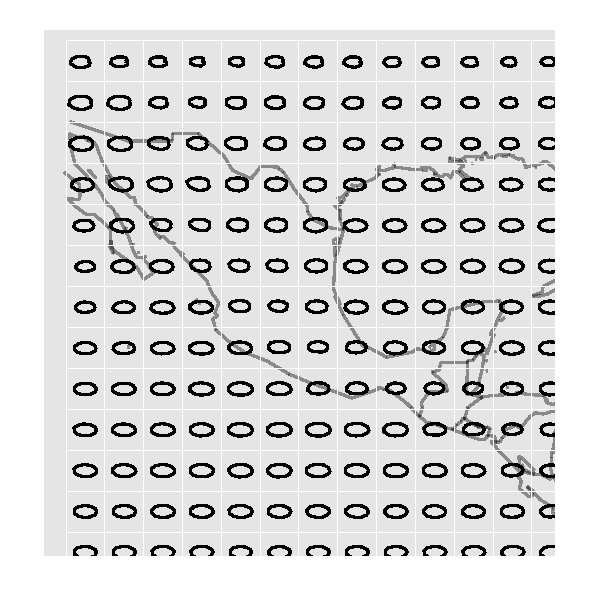
\includegraphics[width=2in]{month-polar}
    
  \caption{Monthly averages in (left) Cartesian coordinates and (right) polar coordinates.}
  
  \label{fig:cycle}
\end{figure}

\section{Generalization: scatterplots}

So far we have limited ourselves to always mapping some aspect of time on the x-axis. But glyph-maps are not limited to only this type of data and can  be easily generalized to create many other types of display. Figure~\ref{fig:cloud} shows a generalisation to scatterplots: by mapping another variable to the x-axis, in this case low-cloud level on x and high-cloud level on y, we can explore how a bivariate relationship varies spatially. It is again useful to use a model to extract the essence of the relationship, summarizing the data with models is very useful: the second plot displays a loess curve fit to the data instead of the individual points.  

\begin{figure}[htbp]
  \centering
  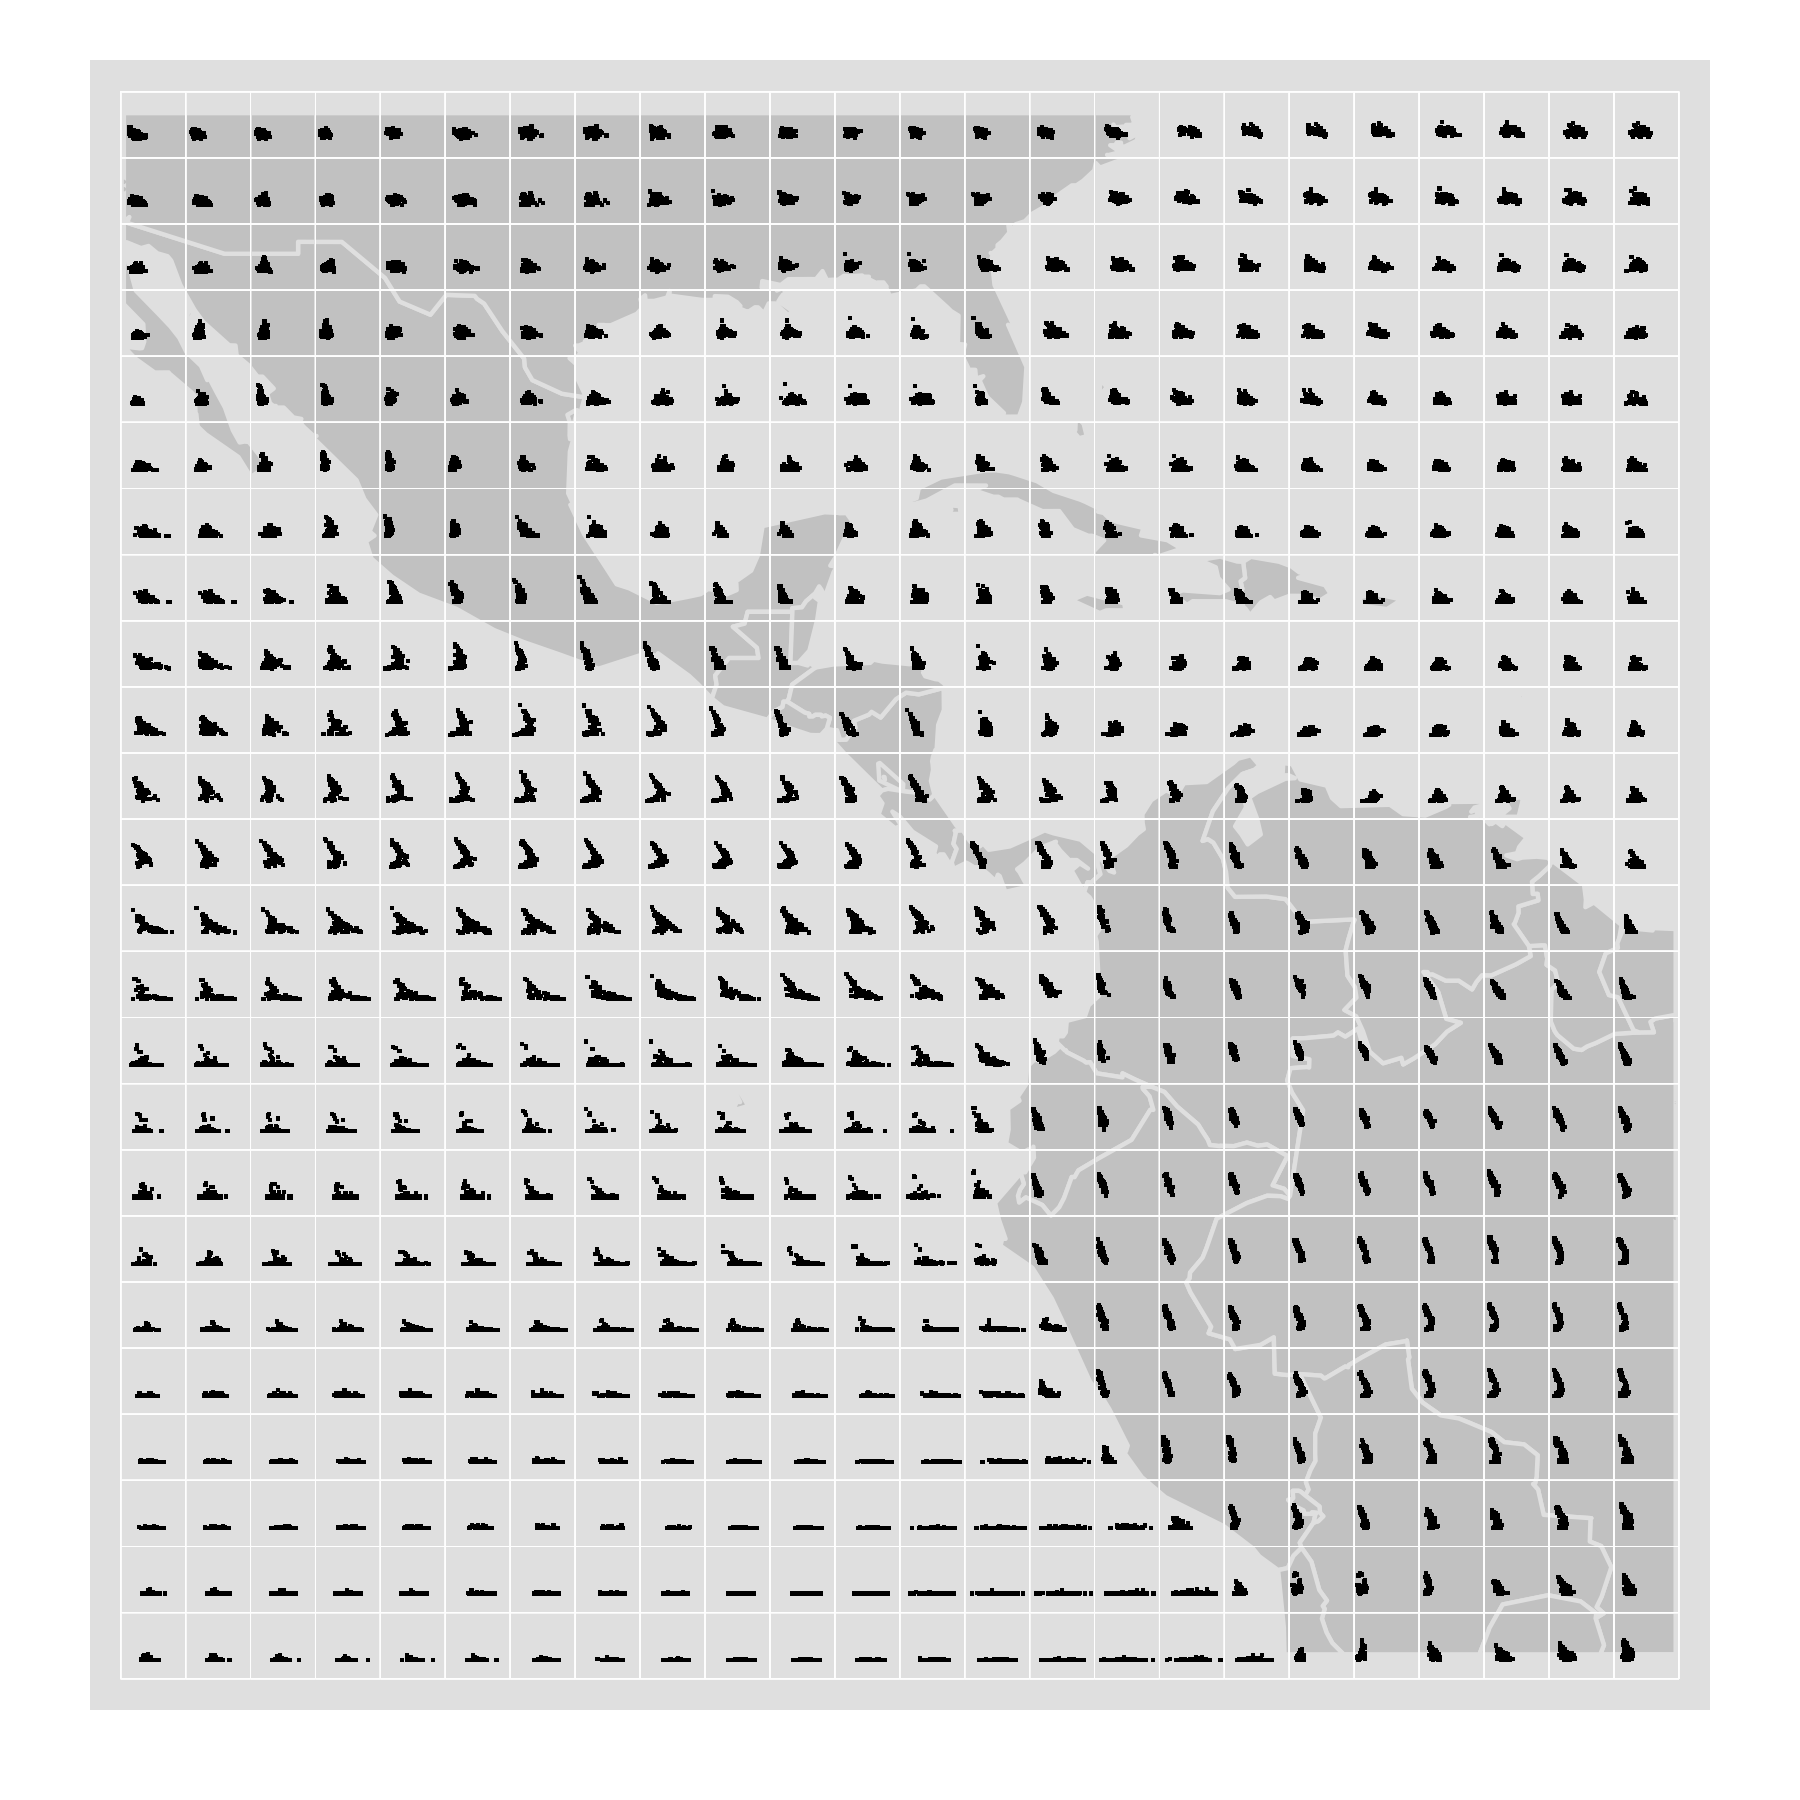
\includegraphics[width=0.5\linewidth]{clouds}%
  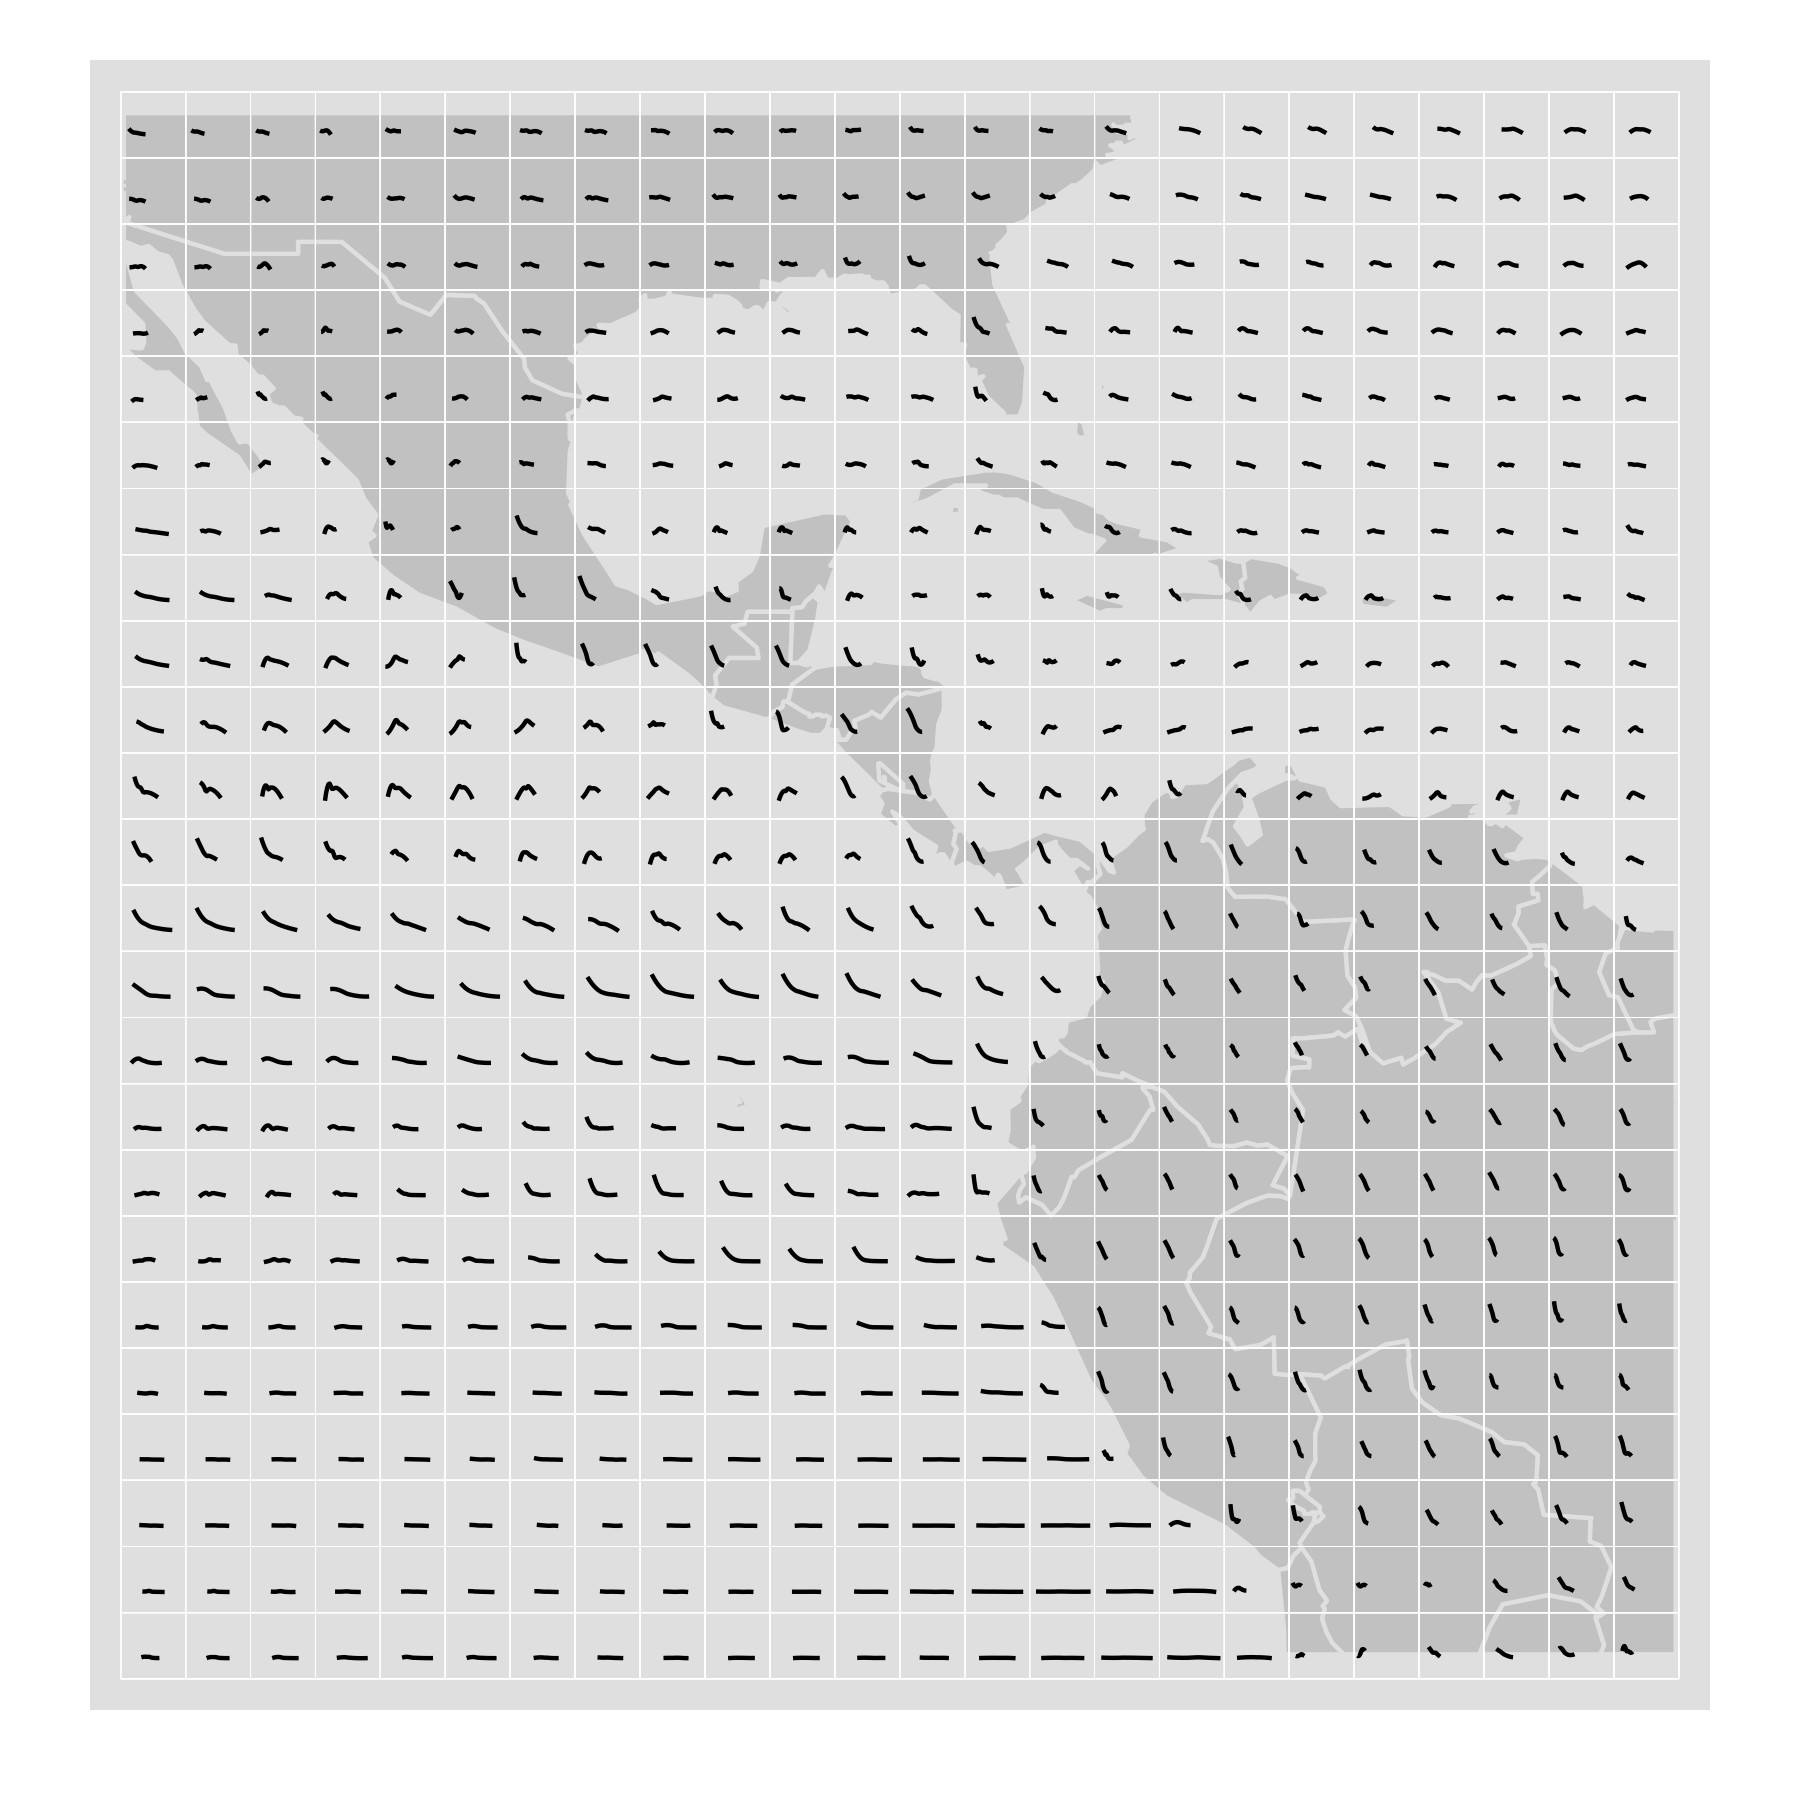
\includegraphics[width=0.5\linewidth]{clouds-smooth}

  \caption{Glyph-map showing (left) scatterplot of high-cloud vs. low-cloud and (right) smoothed (loess) curve fit to each location. The relationship between these two variables varies considerably over the spatial domain (particularly between land and ocean), but neighbouring locations tend to similar. }
  \label{fig:cloud}
\end{figure}

\section{Partitioning patterns into shape and size}

Partitioning is a extremely useful technique: product plots, ANOVA, ...  For glyph plots, it's often useful to partition the glyphs into shape and scale components, decomposing the values into a product of maximum and scaled values. This is revealing for smooth models of surface temperature.

\begin{figure}[htbp]
  \centering
  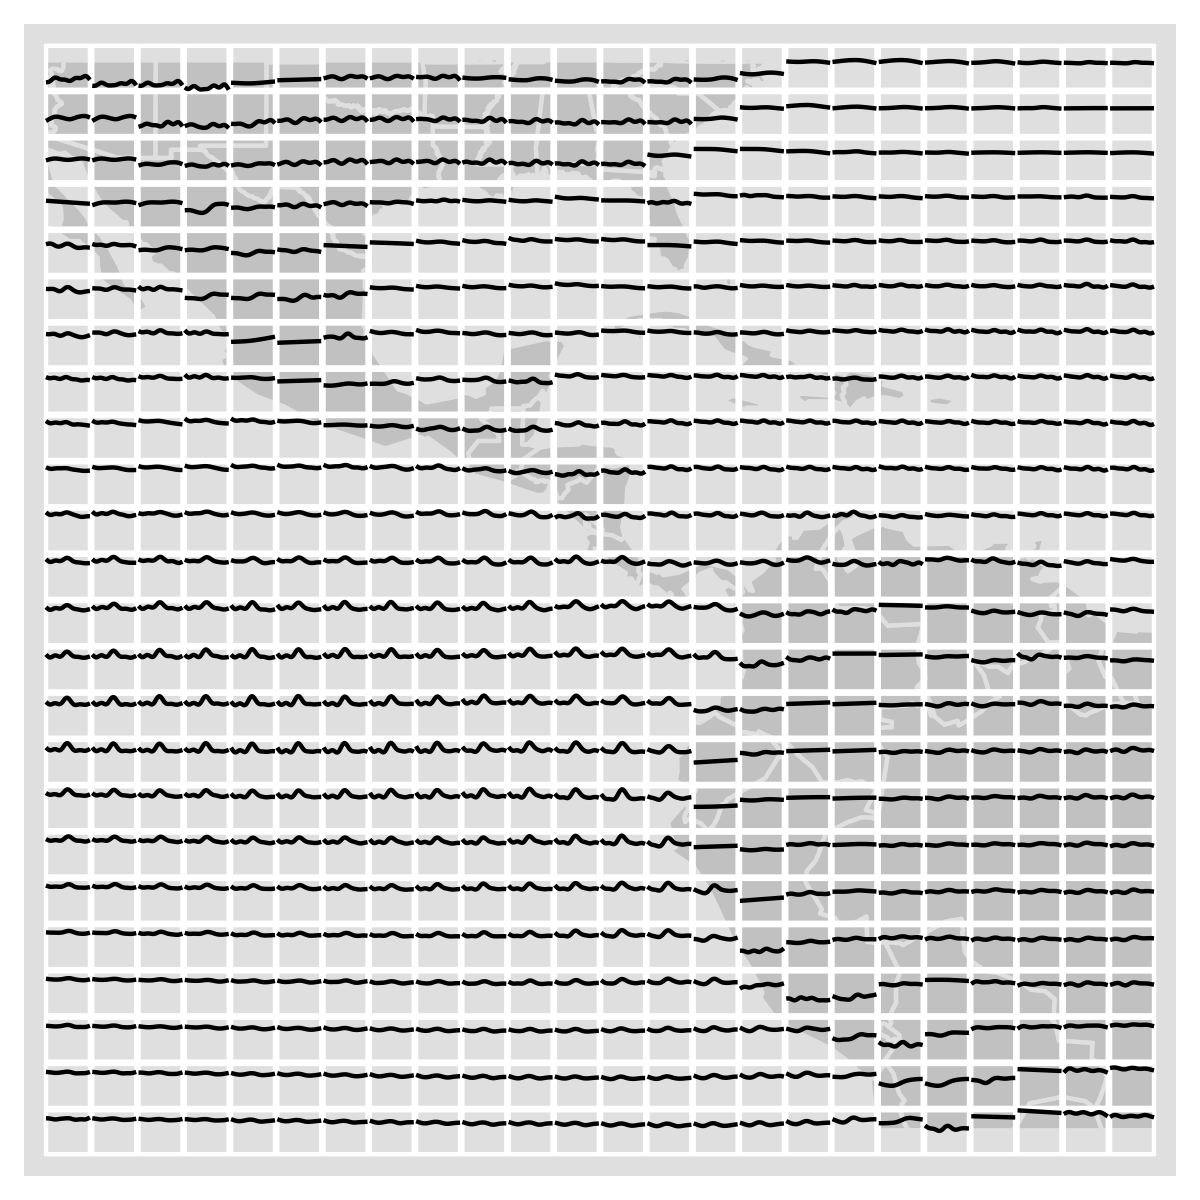
\includegraphics[width=0.33\linewidth]{month-rescale-none}%
  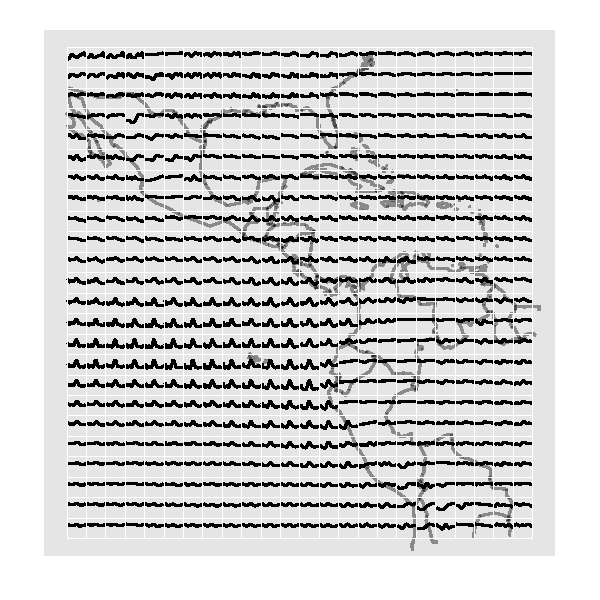
\includegraphics[width=0.33\linewidth]{month-rescale-max}%
  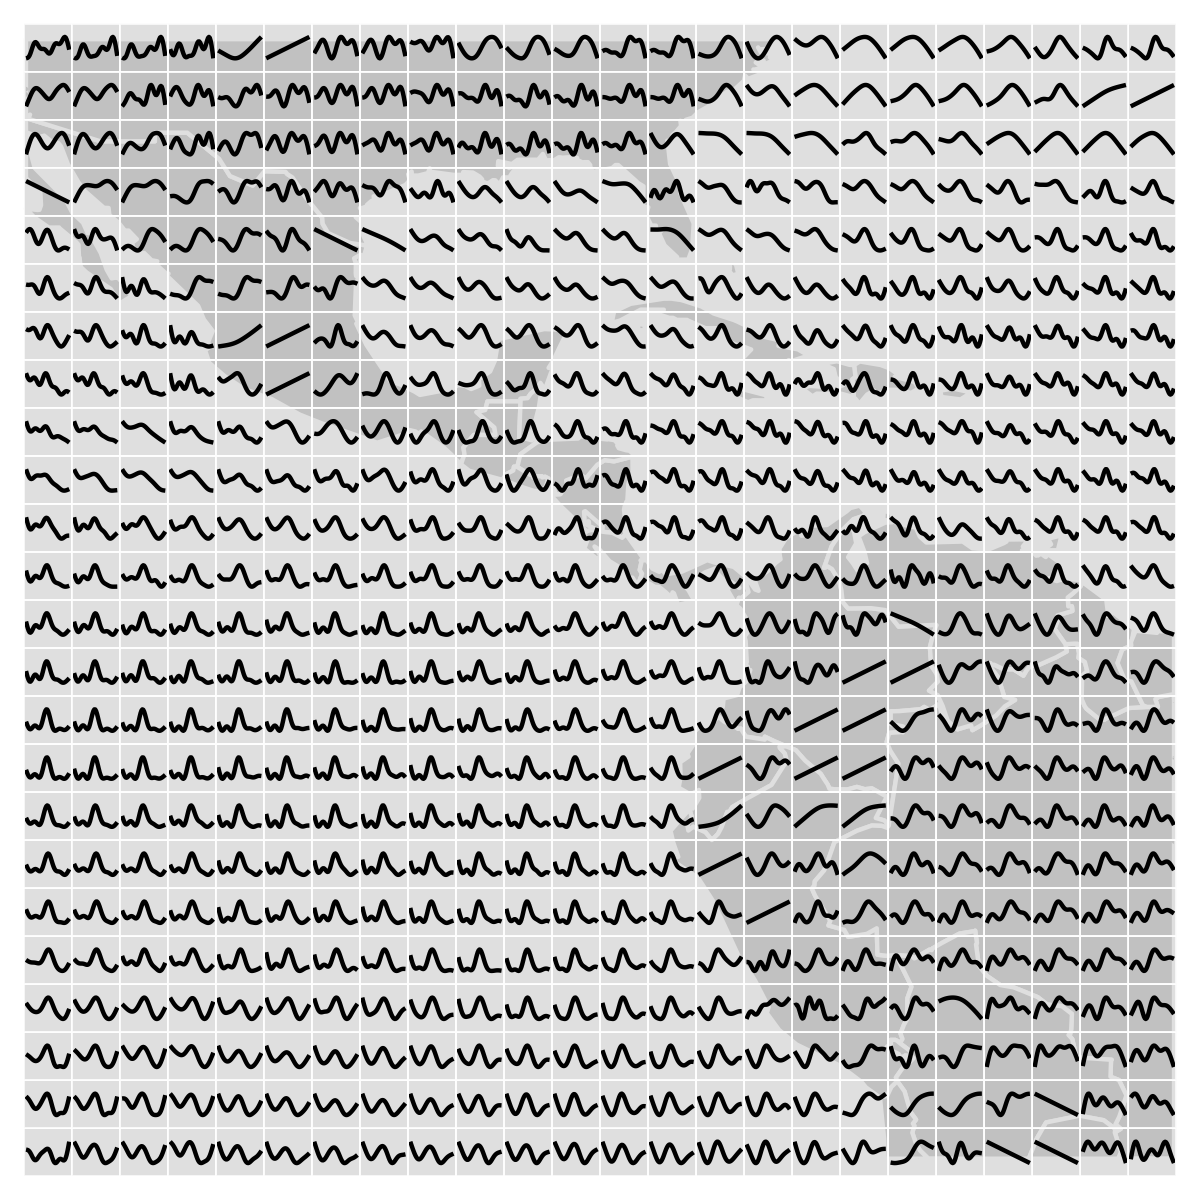
\includegraphics[width=0.33\linewidth]{month-rescale01}
  \caption{Smoothed de-seasonalized daily temperature glyph-map. (Left) unscaled, (center) scaled to have maximum 1, (right) scaled to have maximum 1 and minimum 0.}
  \label{fig:label}
\end{figure}

Of course other types of scaling are possible. Another classical scaling method is to standardize mean and standard deviation to 0 and 1 (or robust variants).

Equivalent to using individual scales in facetted graphics.


\section{Regular vs irregular locations}

\subsection{Non-rectangular grids}

Rectangular, but not in this projection.  Other types of regular grids.

\subsection{Irregular locations}

\section{Conclusions}

\bibliography{references}

\end{document}